\section{Developing multilayer community detection algorithm}
\label{metric}
In this section, first we develop the modularity index $Q_M$ to characterize the quality of multilayer communities. Next, we show
that simple adaptation of $Q_M$ with classical methodologies may lead to the development of multilayer community detection algorithms.

%the way we combine it with existing single layer community detection algorithms to detect multilayer communities.
% \begin{figure*}
% \centering
% 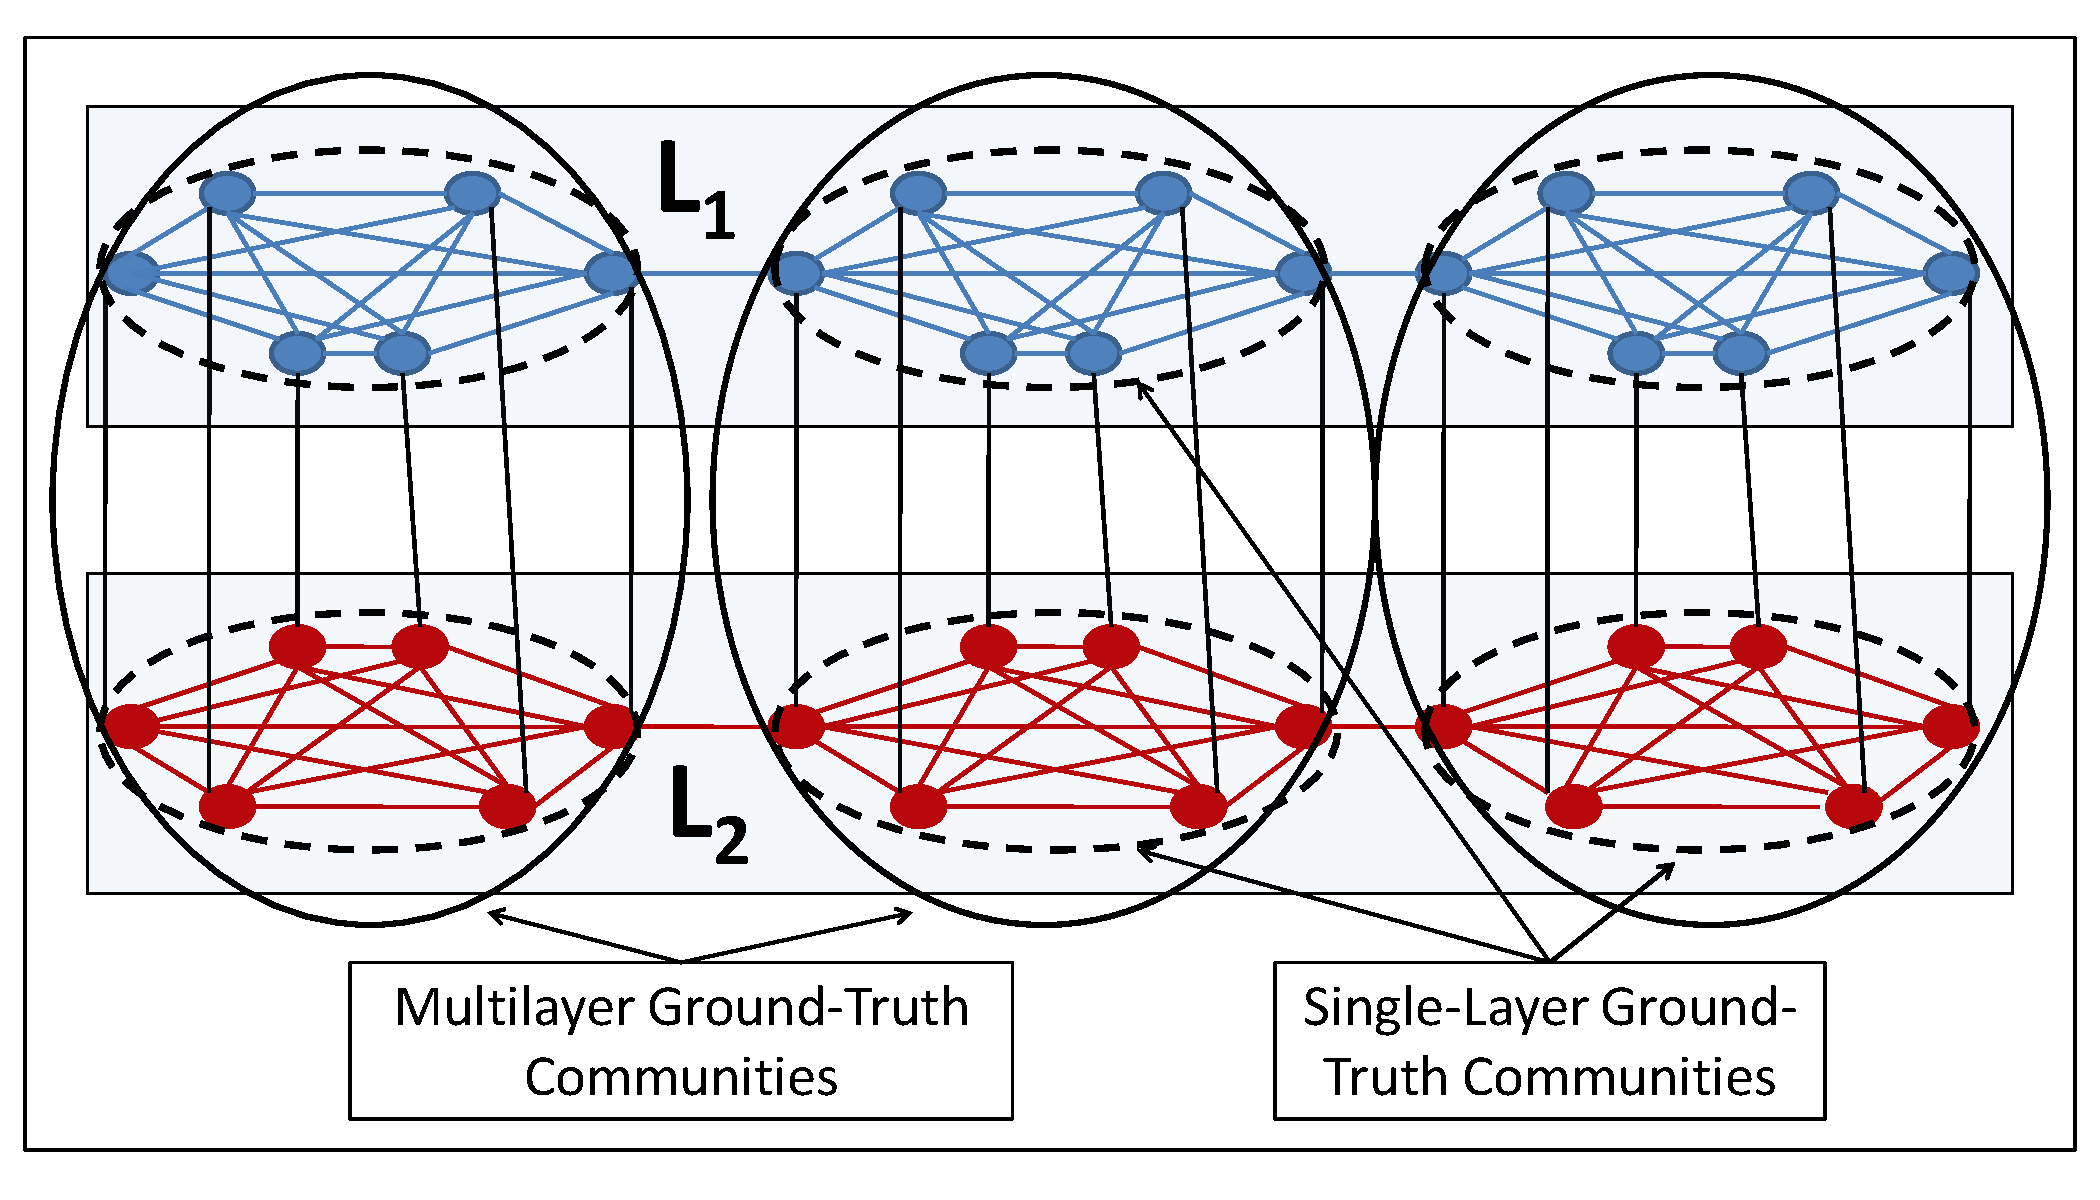
\includegraphics[width=3.5in]{./images/image31.pdf}
% \vspace{-0.2in}
% \caption{Network configuration with two different ground truth communities}
% \vspace{-0.2in}
% \label{N0}
% \end{figure*}

% \begin{figure}
% \centering
% 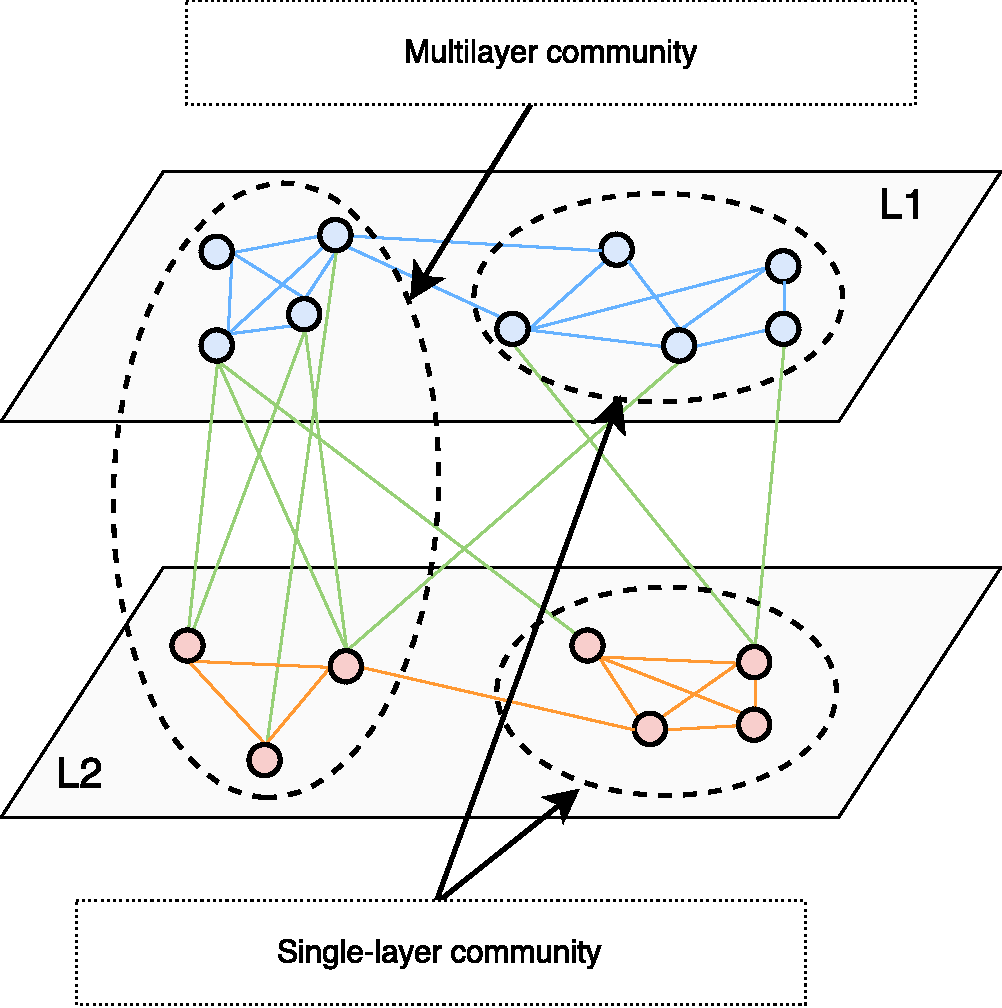
\includegraphics[width=2in]{./images/single_multi_community.pdf}
% \vspace{-0.1in}
% \caption{A sample multilayer network with two different types of communities}
% \label{mul_comm}
% \end{figure}

\subsection{Desired properties of multilayer communities: Intuition}\label{prop}
We start this section highlighting the desired properties of the communities in a multilayer network.
As introduced in section~\ref{dataset}, in multilayer networks, we observe two types of communities (see Fig.~\ref{N0})
(a) cross layer communities (containing multiple types of nodes) and
(b) single layer communities (containing only single type of nodes).

For an `ideal' cross layer community $C = (\mathcal{C_U},\mathcal{C_B})$ of $\mathcal{G}$
(where $\left \vert \mathcal{C_B} \right \vert \neq \Phi$), the desired properties are the following,

\textbf{$Property^{X1}:$} The group of nodes in each uni-partite and bipartite layer ($L^C_i$s and $L^C_{ij}$s respectively) should 
be highly cohesive.

\textbf{$Property^{X2}:$} The (coupling) edges in the bipartite layer $L^C_{ij} \in \mathcal{C_B}$ should connect most of the nodes
from $L^C_i$ (i.e. $V^C_i$) with most of the nodes from $L^C_j$ (i.e. $V^C_j$).

%For each pair of $(L^C_i, L^C_j) \in \mathcal{C_U}$,

Similarly, for an `ideal' single layer community $C= (\mathcal{C_U},\mathcal{C_B})$ of $\mathcal{G}$ (where
$\mathcal{C_B} = \Phi$), the desired properties are enumerated below,

\textbf{$Property^{S1}:$} The community should be highly cohesive within the layer $L_i$ to which it
belongs (i.e. $\mathcal{C_U} = L^C_i \subseteq L_i$).

\textbf{$Property^{S2}:$} The nodes in $L^C_i$ (i.e. $V^C_i$) should be very loosely connected with nodes of other layers $L_j$.

%\vspace{-0.4in}
\subsection{Multilayer Modularity Index}\label{mult_mod}
Following the aforesaid intuitions, we propose multilayer modularity for a two-layer network
$\mathcal{G} = \{\{L_1, L_2\}, \{L_{12}\}\}$
where $L_1$ = ($V_1$, $E_1$) \& $L_2$ = ($V_2$, $E_2$) are the individual layers
and $L_{12}$ = ($V_1$, $V_2$, $E_{12}$) is the bipartite graph connecting nodes of layer $L_1$ and $L_2$.

We start with the basic notion of Newman-Girvan modularity~\cite{newman2006modularity},
$Q = \frac{1}{2m}\sum_{i,j} (A_{ij} - P_{ij})\delta(\psi_i,\psi_j)$ where $m$
%$= \left \vert E_1 \right \vert + \left \vert E_2 \right \vert + \left \vert E_{12} \right \vert$
is the total number of edges in the network, $i,j \in V_1 \cup V_2$ are any pair of nodes in the
network, $\psi_i$ indicates the community membership of node $i$ and $\delta(\psi_i,\psi_j)$ is the Kronecker delta function which
is $1$ only if $\psi_i=\psi_j$ i.e. $i$ and $j$ belong to the same community (and $0$ otherwise).
%[BM: notational inconsistency with $c_i$, community or coupling degree?]
$A_{ij}$ represents the classical adjacency matrix of $\mathcal{G}$. The penalty term $P_{ij}$ (often referred as null model)
is the expected probability of having an edge between nodes $i$ and $j$ if edges are placed at random.
Notably, in multilayer network the edges in one layer $L_i$ are intrinsically different from another layer $L_j$, which gets
reflected in the property of the corresponding layers as well (say diverse edge densities across the layers). This observation motivates
us to introduce layer-wise discriminating null models, and propose the following
multilayer modularity, %[BM: try if this can be part of Eq 1] $Q_M= \frac{1}{2m}\sum_{ij}\{(A_{ij}-P_{ij})\delta(\psi_i,\psi_j)\}~where$
\vspace{-0.1in}
\begin{dmath}\label{eq11}
{Q_M = \frac{1}{2m}\sum_{ij}\{(A_{ij}-P_{ij})\delta(\psi_i,\psi_j)\} ~where}\\
{P_{ij}=\left\{ \begin{array}{ll}
                  P^1_{ij}~~if~i \in V_1~\&~j \in V_1\\
                  P^2_{ij}~~if~i \in V_2~\&~j \in V_2\\
                  P^{12}_{ij}~~if~(i \in V_1~\&~j \in V_2)~or~(i \in V_2~\&~j \in V_1)
                \end{array}
              \right.}
\end{dmath}
\vspace{-0.15in}
In the following, we compute the null model terms $P^1_{ij}$, $P^2_{ij}$ and $P^{12}_{ij}$ separately for both types
of communities of multilayer network and finally derive the multilayer modularity index $Q_M$.
%in a way that imposes our desired behaviours (as discussed in the previous subsection) on them.
% As mentioned before, we have a very different set of expectations from a cross layer community than a single layer one.
% Due to this fact, the $P^1_{ij}$, $P^2_{ij}$ and $P^{12}_{ij}$ terms have to be defined separately for both type of communities.

\subsubsection{Cross Layer Communities}
Any cross layer community $C$ is composed of three submodules - two intra layer ($L^C_1$, $L^C_2$) and one inter layer ($L^C_{12}$).
The vanilla null model proposed in~\cite{newman2006modularity} directly derives the $P^1_{ij}$, $P^2_{ij}$ for intra layer submodules.
The expected number of edges between any two nodes $i$ and $j$ (with intra-layer degrees
$h_i$ and $h_j$ respectively) within the community $C$ can be calculated as
$P^1_{ij}=(h_i*h_j)/2\left \vert E_1 \right \vert$ (for submodule $L^C_1$) and $P^2_{ij}=(h_i*h_j)/2\left \vert E_2 \right \vert$
(for submodule $L^C_2$).
%This is essentially the same classic null model proposed by Newman~\cite{newman2006modularity}.
For inter layer or bipartite submodule $L^C_{12}$, the probability of an edge between node $i$ and $j$ depends on their respective
coupling degrees $c_i$ and $c_j$.
%not only depends on their degrees in the corresponding coupling layer but
%also on their individual intra-layer degrees.
The probability of having a coupling edge between $i$, $j$ can be estimated as $P^{12}_{ij}=(c_i*c_j)/\left \vert E_{12} \right
\vert$ (similar
to~\cite{barber2007modularity}). The aforementioned null models satisfy the desired requirements of $Property^{X1}$ introduced
in section~\ref{prop}.
%[SP:SHOULD I REFER BARBAR's MODULARITY?].

Each cross layer community $C$ is represented as $\{\{L^C_1, L^C_2\}, \{L^C_{12}\}\}$ where
$L^C_1$ and $L^C_2$ are the submodules with edges from $E_1$ and $E_2$ respectively and $L^C_{12}$ is from $E_{12}$;
we substitute $P_{ij}$ in Eq.~\ref{eq11} to define its modularity as
\vspace{-0.1in}
\begin{dmath}\label{eq_mid}
Q_M^C= {\forall i,j \in C}~ \left[ \frac{1}{3} \bigg \{
 \frac{1}{2\left \vert E_1 \right \vert}
 \sum_{i,j \in V_1}\big(A_{ij} - \frac{ (h_i * h_j)}{2\left \vert E_1 \right \vert}\big) +
 \frac{1}{\left \vert E_{12} \right \vert}
 \sum_{i \in V_1, j \in V_2}\big(A_{ij} - \frac{ (c_i * c_j)}{\left \vert E_{12} \right \vert}\big) +
 \frac{1}{2\left \vert E_{2} \right \vert}
 \sum_{i,j \in V_2}\big(A_{ij} - \frac{ (h_i * h_j)}{2\left \vert E_2 \right \vert}\big)
    \bigg \}\right]
\end{dmath}
\vspace{-0.08in}
% Q_M^C= \forall i,j \in C~ \{\frac{1}{3}\{(\frac{\sum_{i,j \in V_1} A_{ij}}{2*\left \vert E_1 \right \vert} -
%  \frac{\sum_{i,j \in V_1} (h_i * h_j)}{(2*\left \vert E_1 \right \vert)^2}) +
%  (\frac{\sum_{L(i) \neq L(j)} A_{ij}}{2*\left \vert E_{12} \right \vert} -
%  \frac{\sum_{L(i) \neq L(j)} (c_i * c_j)}{2*\left \vert E_{12} \right \vert^2}) +
%  (\frac{\sum_{i,j \in V_2} A_{ij}}{2*\left \vert E_2 \right \vert} -
%  \frac{\sum_{i,j \in V_2} (h_i * h_j)}{(2*\left \vert E_2 \right \vert)^2})\}\}
%where $L(i)=l$ if vertex $i$ belongs to layer $l$.
%[BM: be consistent in the terminologies. intra-layer submodule or bipartite submodule? edge/edges etc]
% \begin{dmath}
% OR,~Q_M^C= \forall i,j \in C~ \{\frac{1}{3}\{(\frac{\sum_{i,j \in V_1} A_{ij}}{2*\left \vert E_1 \right \vert} -
%  \frac{(\sum_{i \in V_1} h_i) * (\sum_{j \in V_1} h_j)}{(2*\left \vert E_1 \right \vert)^2}) +
%  (\frac{\sum_{i \in V_1 j \in V_2} A_{ij}}{\left \vert E_{12} \right \vert} -
%  \frac{(\sum_{i \in V_1} c_i) * (\sum_{j \in V_2} c_j)}{(\left \vert E_{12} \right \vert)^2}) +
%  (\frac{\sum_{i,j \in V_2} A_{ij}}{2*\left \vert E_2 \right \vert} -
%  \frac{\sum_{i \in V_2} h_i * \sum_{j \in V_2} h_j}{(2*\left \vert E_2 \right \vert)^2})\}\}
% \end{dmath}
%[BM: one sum per layer.]
In case of inter layer submodule, if node $i$ in $C$ is not connected with any other layer (hence, coupling degree $c_i$ zero), we
use its intra layer degree $h_i$ as a proxy of $c_i$ for computing $P^{12}_{ij}$. This allows us to penalize those
nodes in cross layer community $C$ which are only connected with
nodes within the same layer and \emph{not} with the nodes in $C$ of different layer. This amendment in the null
model $P^{12}_{ij}$ satisfies the desired requirements of $Property^{X2}$. Therefore with this modification, the Eq.~\ref{eq_mid}
can be written as,
\vspace{-0.08in}
\begin{dmath}\label{eq_multi}
Q_M^C= {\forall i,j \in C}~  \left[ \frac{1}{3}\bigg \{
 \frac{1}{2\left \vert E_1 \right \vert}
 \sum_{i,j \in V_1}\big(A_{ij} - \frac{ (h_i * h_j)}{2\left \vert E_1 \right \vert}\big) +\\
 {\frac{1}{2\left \vert E_1 \right \vert + 2\left \vert E_2 \right \vert + \left \vert E_{12} \right \vert}
 \sum_{i \in V_1, j \in V_2}\big(A_{ij} - \frac{ ({c'}_i * {c'}_j)}
 {2\left \vert E_1 \right \vert + 2\left \vert E_2 \right \vert + \left \vert E_{12} \right \vert}\big)} +
 \frac{1}{2\left \vert E_{2} \right \vert}
 \sum_{i,j \in V_2}\big(A_{ij} - \frac{ (h_i * h_j)}{2\left \vert E_2 \right \vert}\big)
   \bigg \}\right]
\end{dmath}
\vspace{-0.08in}
where for any node $i$, ${c'}_i=c_i$ if $c_i > 0$ and ${c'}_i=h_i$ otherwise.
% [BM: rewrite the following sentence?? I tried once.]
% Finally, summing over all node pairs in the community $C$ following Eq.~\ref{eq_mid},
% \begin{dmath}\label{cross1}
% Q_M^C= \{\frac{1}{3}\{\underbrace{[\frac{\left \vert E^C_1 \right \vert}{\left \vert E_1 \right \vert}-
%  (\frac{d^C_1}{2*\left \vert E_1 \right \vert})^2]}_{Term~ for~ Single~ Layer~ L_1}
%  +\underbrace{[\frac{\left \vert E^C_{12} \right \vert}{\left \vert E_{1} \right \vert + \left \vert E_{2} \right \vert + \left \vert E_{12} \right \vert}-
%  \frac{k^C_{12}*{d^C_{12}}}{{(2*\left \vert E_{1} \right \vert + 2*\left \vert E_{2} \right \vert + \left \vert E_{12} \right \vert)}^2}]}_{Term~ for~ Coupling~ edges}
%  +\underbrace{[\frac{\left \vert E^C_2 \right \vert}{\left \vert E_2 \right \vert}-(\frac{d^C_2}{2*\left \vert
%  E_2 \right \vert})^2]}_{Term~ for~ Single~ Layer~ L_2}\} \}
% \end{dmath}
% where $\left \vert E^C_1 \right \vert$, $\left \vert E^C_2 \right \vert$ \& $\left \vert E^C_{12} \right \vert$ are the number of edges
% present in community $C$ from layers $L_1$, $L_2$ and $L_{12}$; $d^C_1$ ($d^C_2$) is the sum of intra-layer degrees of
% all $L^C_1$ ($L^C_2$) nodes in $L_1$ ($L_2$) layer;
% $k^C_{12}$ and $d^C_{12}$ [BM: change the symbols $k, d$] are the sum of coupling degrees (with suitable proxies)
% of $L^C_1$ and $L^C_2$ nodes respectively.

%and $d^C_{12}$ is the sum of coupling degrees of $L^C_2$ nodes.
%in subnetwork $L_{12}$.


\subsubsection{Single Layer Communities}
In any single layer community $C$, all the constituent nodes belong to either $L_1$ or $L_2$. The null models
can be directly derived as $P^1_{ij}=(h_i*h_j)/2\left \vert E_1 \right \vert$ and $P^2_{ij}=(h_i*h_j)/2\left \vert E_2 \right \vert$ for
layer $L_1$ and $L_2$ respectively from the vanilla null model~\cite{newman2006modularity}. These null models satisfy
the $Property^{S1}$ introduced in section~\ref{prop}.
Hence, for each single layer community $C$ represented as $\{L^C_1\}$,
we substitute $P_{ij}$ in Eq.~\ref{eq11} to compute the modularity as,
\vspace{-0.05in}
\begin{dmath}
Q_M^C={\forall i,j \in C} \left [ \frac{1}{3} \bigg \{
\frac{1}{2\left \vert E_1 \right \vert} \sum_{i,j \in V_1}
\big(A_{ij} -
\frac{(h_i * h_j)}{2\left \vert E_1 \right \vert}\big) \bigg \} \right]  \end{dmath}
\vspace{-0.05in}
Importantly, there can be many nodes in $C$ which are connected to other layer nodes via coupling edges,
violating $Property^{S2}$ of desired single layer community.
%one of our desired criteria (loose coupling with nodes from the other layer) for an `ideal' single layer community.
In order to penalize those nodes in a community $C$ with coupling
degree $c_i$, we add $c_i$ along with $h_i$ to estimate the null model.
Subsequently, the modularity of $C$ becomes
%After taking care of the coupling degrees of nodes in a single layer community,
\vspace{-0.05in}
\begin{dmath}\label{eq_single}
{Q_M^C=\forall i,j \in C}~ \penalty0{\left[ \frac{1}{3} \bigg \{
\frac{1}{2\left \vert E_1 \right \vert+\left \vert E_{12} \right \vert} \sum_{i,j \in V_1}
\big(A_{ij} - \penalty0
\frac{(h_i+c_i) * (h_j+c_j)}{2\left \vert E_1 \right \vert+\left \vert E_{12} \right \vert}\big) \bigg \}
\right]}
\end{dmath}
\vspace{-0.08in}
% Q_M^C=\forall i,j \in C~ \{\frac{1}{3}(\frac{\sum_{i,j \in V_1} A_{ij}}{2*\left \vert E_1 \right \vert+\left \vert E_{12} \right \vert} -
%  \frac{\sum_{i,j \in V_1} ((h_i+c_i) * (h_j+c_j))}{(2*\left \vert E_1 \right \vert+\left \vert E_{12} \right \vert)^2}) \}

%This reflects the fact that a node with high coupling degree can only be a part of a single layer community if it contributes even higher number of edges within the community which essentially imposes our desired criteria.

%Notably, it is not required to add this type of coupling degree terms while calculating single layer modularities of cross layer communities because Eq.~\ref{cross1} already has a bipartite term to take care of them judiciously.

% \begin{dmath}
% OR,~Q_M^C= \forall i,j \in C~ \{\frac{1}{3}(\frac{\sum_{i,j \in V_1} A_{ij}}{2*\left \vert E_1 \right \vert+\left \vert E_{12} \right \vert} -
%  \frac{(\sum_{i \in V_1} (h_i+c_i)) * (\sum_{j \in V_1} (h_j+c_j))}{(2*\left \vert E_1 \right \vert+\left \vert E_{12} \right \vert)^2}) \}
% \end{dmath}
% But they may or may not be connected
% with other layer vertices via coupling edges. So, the expected number of edges between $i$ and $j$ with intra-layer degrees
% $h_i$ \& $h_j$ and coupling degrees $c_i$ \& $c_j$ can be calculated as
% $((h_i+c_i)*(h_j+c_j))/2\left \vert E_1 \right \vert$ or $((h_i+c_i)*(h_j+c_j))/2\left \vert E_2 \right \vert$ depending on whether
% the community is in layer 1 or layer 2.
% Finally, summing over all node pairs in the community $C$ following Eq. XX [BM: replace],
% \begin{dmath}
% Q_M^C= \{\frac{1}{3}(\frac{\left \vert E^C_1 \right \vert}{\left \vert E_1 \right \vert+ \left \vert E_{12} \right \vert/2}-
%  (\frac{{d'}^C_1}{2*\left \vert E_1 \right \vert+\left \vert E_{12} \right \vert})^2) \}
% \end{dmath}
% where $\left \vert E^C_1 \right \vert$ is the number of intra community edges and ${d'}^C_1 = {d}^C_1 + {CO}^C_1$ is the sum of intra-layer (${d}^C_1$) and coupling (${CO}^C_1$) degrees of
% all $L^C_1$ nodes in $L_1$ layer. Similar expression can be derived if $C$ is a submodule of $L_2$.

Finally, combining both types of communities, the overall modularity of the network can be represented as
\vspace{-0.07in}
\begin{dmath}\label{final1}
Q_M= \frac{1}{3}\sum_{k=1}^{n_C}\left[ {\forall i,j \in C_k}~\penalty0   \bigg \{
 \frac{1}{2\left \vert E_1 \right \vert + \theta_{C_k}*\left \vert E_{12} \right \vert }
 \sum_{i,j \in V_1}\big(A_{ij} - \\   {     \frac{ (h_i+\theta_{C_k}*c_i) * (h_j+\theta_{C_k}*c_j)}
 {2\left \vert E_1 \right \vert+ \theta_{C_k}*\left \vert E_{12} \right \vert}\big) +
 \frac{1}{2\left \vert E_1 \right \vert + 2\left \vert E_2 \right \vert + \left \vert E_{12} \right \vert}} \penalty0
 \sum_{i \in V_1, j \in V_2}\big(A_{ij} - \frac{ ({c'}_i * {c'}_j)}
 {2\left \vert E_1 \right \vert + 2\left \vert E_2 \right \vert + \left \vert E_{12} \right \vert}\big) +
 \frac{1}{2\left \vert E_{2} \right \vert+ \theta_{C_k}*\left \vert E_{12} \right \vert} \penalty0
 \sum_{i,j \in V_2}\big(A_{ij} -
 \frac{ (h_i+\theta_{C_k}*c_i) * (h_j+\theta_{C_k}*c_j)}{2\left \vert E_2 \right \vert +
 \theta_{C_k}*\left \vert E_{12} \right \vert}\big)
   \bigg \} \right]
\end{dmath}
\vspace{-0.1in}
%   Q_M=\frac{1}{3}\sum_{C=1}^{n_C}\{\underbrace{[\frac{\left \vert E^C_1 \right \vert}
%   {\left \vert E_1 \right \vert + \theta_{C_k}*(\left \vert E_{12} \right \vert/2)}-
%  (\frac{d^C_1+\theta_{C_k}*{CO}^C_1}{2*\left \vert E_1 \right \vert + \theta_{C_k}*\left \vert E_{12} \right \vert})^2]}_{Term~ for~ Single~ Layer~ L_1}
%  +\underbrace{[\frac{\left \vert E^C_{12} \right \vert}{\left \vert E_{1} \right \vert + \left \vert E_{2} \right \vert + \left \vert E_{12} \right \vert}-
%  \frac{k^C_{12}\times{d^C_{12}}}{{(2*\left \vert E_{1} \right \vert + 2*\left \vert E_{2} \right \vert + \left \vert E_{12} \right \vert)}^2}]}_{Term~ for~ Coupling~ edges}
%  +\underbrace{[\frac{\left \vert E^C_2 \right \vert}{\left \vert E_2 \right \vert + \theta_{C_k}*(\left \vert E_{12} \right \vert/2)}
%  -(\frac{d^C_2+\theta_{C_k}*{CO}^C_2}{2*\left \vert
%  E_2 \right \vert + \theta_{C_k}*\left \vert E_{12} \right \vert})^2]}_{Term~ for~ Single~ Layer~ L_2}\}

where $n_C$ is the total number of apriori communities and $\theta_{C_k}$ is a variable denoting type of the community $C_k$. $\theta_{C_k}$
is $1$ if $C_k$ is a single layer community and $0$ if $C_k$ is a cross layer community.
Notably, for any single layer community, maximum one of the single layer terms in Eq.~\ref{final1} can be non-zero; the other
two terms will always be zero.
\vspace{-0.1in}
\begin{algorithm} \small

    \DontPrintSemicolon
    \SetKwInOut{Input}{Input}
    \SetKwInOut{Output}{Output}
    \SetKwProg{Fn}{Function}{:}{}
     \Input{A multilayer network $\mathcal{G}$ as defined in section~\ref{mult_mod} where $E= E_1 \cup E_2 \cup E_{12}$.}
     %where $E$ is the set of all intra and inter layer edges in $\mathcal{G}$.}
     \Output{Maximum $Q_M$ of $\mathcal{G}$ and detected communities.}

     Calculate the betweenness centralities of all edges\;
     \While{$\left \vert E \right \vert > 1$}{
      Remove the edge $e \in E$ with maximum betweenness centrality from $E$\;
      $currQ$ = current $Q_M$ of $\mathcal{G}$\;
      Save the current partition along with $currQ$\;
      Update the betweenness centralities of remaining edges\;
     }
     Display partition with maximum $Q_M$\;
     \KwRet\;

\caption{GN-$Q_M$} %Algorithm to map Meetup venues with Yelp venues}
\label{algo3}
\end{algorithm}
\vspace{-0.1in}

Although, we show the derivation of $Q_M$ for a two layer network, it can be easily extended for more
than two layers. For instance, if the network has $L$ layers with $L-1$ coupling relationships between them, there would be
$L$ single layer and $L-1$ bipartite modularity terms in the corresponding $Q_M$ equation.
% % We start with a simplistic metric considering a linear combination of Newman-Girvan modularity for simple graph~\cite{newman2004finding}
% % and Barber modularity for bipartite graph~\cite{barber2007modularity}.
% % ,
% % we can represent the modularity index as
% % \begin{equation}\label{eqn1}
% % %\resizebox{\columnwidth}{!}{
% %  mQ=\frac{1}{3}\sum_{C=1}^{n_C}\{\underbrace{[\frac{\left \vert E^C_1 \right \vert}{\left \vert E_1 \right \vert}-
% %  (\frac{d^C_1}{2\left \vert E_1 \right \vert})^2]}_{Term~ for~ Single~ Layer~ L_1}
% %  +\underbrace{[\frac{\left \vert E^C_{12} \right \vert}{\left \vert E_{12} \right \vert}-
% %  \frac{k^C_{12}\times{d^C_{12}}}{{\left \vert E_{12} \right \vert}^2}]}_{Term~ for~ Coupling~ edges}
% %  +\underbrace{[\frac{\left \vert E^C_2 \right \vert}{\left \vert E_2 \right \vert}-(\frac{d^C_2}{2\left \vert
% %  E_2 \right \vert})^2]}_{Term~ for~ Single~ Layer~ L_2}\}
% %  %}
% % \end{equation}
% % %[BM: with underbrace, write - term for single layer $L_1$, term for crosslayer edges, term for single layer $L_2$]
% % where each community $C$ is represented as $\{\{L^C_1, L^C_2\}, \{L^C_{12}\}\}$.
% % %$L^C_1$ and $L^C_2$ are the submodules with edges from $E_1$ and $E_2$ respectively and $L^C_{12}$ is from $E_{12}$;
% % %$I^C_1$ is the number of edges in submodule $L^C_1$ i.e. $I^C_1 = \left \vert E^C_1 \right \vert$,
% % %$m_1$ is the size of subnetwork $G_1$ i.e. ,
% % $n_C$ is the number of apriori communities; $d^C_1$ is the sum of degrees of all $L^C_1$ nodes in $L_1$ layer;
% % $k^C_{12}$ is the sum of degrees of $L^C_1$ nodes in subnetwork $L_{12}$ and $d^C_{12}$ is the sum of
% % degrees of $L^C_2$ nodes in subnetwork $L_{12}$ (identical to~\cite{medical_paper}).
% % % In fact, this definition is basically a linear combination of Newman-Girvan modularity for simple graph~\cite{newman2004finding}
% % % and Barber modularity for bipartite graph~\cite{barber2007modularity}.
% %
% % % where $n_c$ is the number of apriori communities; $I_{Ac}$ is the number of edges within community $L^C_1$, $m_A$ is the size of subnetwork
% % % $G_A$, $d_{Ac}$ is the sum of degrees of all $L^C_1$ nodes in $G_A$; $k_{\pi c}$ is the sum of degrees of A nodes of $\pi c$
% % % in subnetwork $G_\pi$, $d_{\pi c}$ is the sum of degrees of B nodes of $\pi c$ in $G_\pi$. [BM: carefully correct this notations]
% %
% % \subsubsection{Limitation}
% % The major deficiency of modularity $mQ$ comes from the fact that it checks the quality of a multilayer community
% % by individually checking its single layer and bipartite components. It never checks how well the individual single layer components
% % within each cross layer community are connected with each other. We illustrate this limitation with the help of a representative
% % example. In Fig.~\ref{N0}, we consider a synthetic multilayer network with three cohesive groups of single type nodes
% % (say, cliques) at each layer $L_1$ and $L_2$ respectively. A set of coupling edges connect one group of
% % nodes in layer $L_1$ with the corresponding group in layer $L_2$. We consider two different ground truth configurations
% % as shown in Fig.~\ref{N0} - (i) \textbf{Config A:} single-layer communities comprising cohesive groups only (six communities),
% % (ii) \textbf{Config B:} cross layer communities, comprising one group from Layer $L_1$ with another group from
% % layer $L_2$ (three communities). Intuitively, deletion of coupling edges should make the single layer communities
% % in Config A more cohesive, increasing the modularity of Config A, whereas in Config B, it should dilute the cross layer
% % communities decreasing the modularity. However, in Fig.~\ref{single} the plots corresponding to $mQ$ reveal that
% % none of these desired behaviors get captured by the modularity $mQ$; it remains constant throughout the edge deletion regime. Precisely, in Config A the coupling edges
% % do not have any contribution
% % in Eq.~\ref{eqn1} (coupling edge term vanishes), hence $mQ$ remains constant against removal of coupling edges.
% % On the other hand, in Config B, the edge removal only affects the coupling edge term term; however, removal of edges influences
% % the numerator and denominator almost equally, neutralizing the overall effect on $mQ$.
% %
% % % \begin{figure}
% % % \centering
% % % 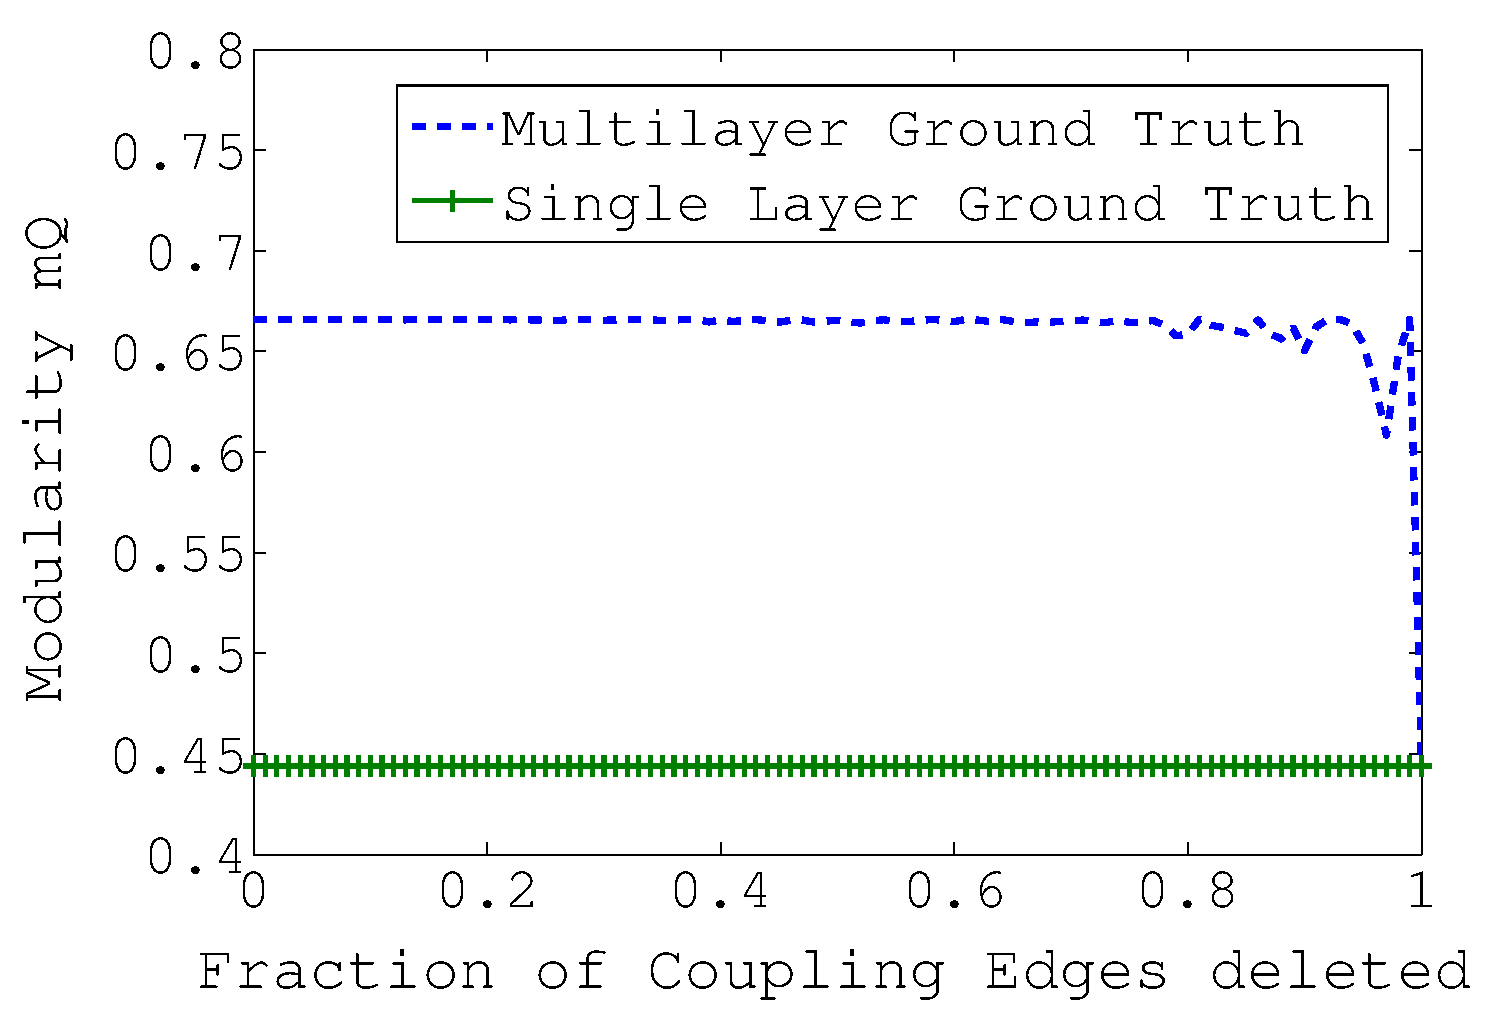
\includegraphics[width=2.5in]{./images/mQ_config1_2_100_5_no_ext_random_removal.pdf}
% % % \vspace{-0.1in}
% % % \caption{Change in mQ while deleting couplinng edges for both ground truth communities in Fig.~\ref{N0}}
% % % \vspace{-0.1in}
% % % \label{mQ1}
% % % \end{figure}
% %
% % \subsubsection{Modularity index $MultiMod$}
% % In order to alleviate the aforesaid limitations of $mQ$, we introduce corrections with each term of it and proposed the following
% % modularity index
% % \begin{dmath}\label{eqn2}
% %  MultiMod=\frac{1}{3}\sum_{C=1}^{n_C}\{[\underbrace{(\frac{\left \vert E^C_1 \right \vert}{\left \vert E_1 \right \vert}-
% %  (\frac{d^C_1}{2\left \vert E_1 \right \vert})^2)}_{Term~ for~ Single~ Layer~ L_1~in~mQ} \times \underbrace{e^{-F^C_1}}_{Correction~ Term}]
% %  +[\underbrace{(\frac{\left \vert E^C_{12} \right \vert}{\left \vert E_{12} \right \vert}-
% %  \frac{k^C_{12}\times{d^C_{12}}}{{\left \vert E_{12} \right \vert}^2})}_{Term~ for~ Coupling~ edges~in~mQ} \times \underbrace{H^C_1\times H^C_2}_{Correction~ Term}]
% %  +[\underbrace{(\frac{\left \vert E^C_2 \right \vert}{\left \vert E_2 \right \vert}-(\frac{d^C_2}{2\left \vert E_2 \right \vert})^2)}_{Term~ for~ Single~ Layer~ L_2~in~mQ}\times \underbrace{e^{-F^C_2}}_{Correction~ Term}]\}
% %  \end{dmath}
% % % \begin{equation}
% % %  mQ=\frac{1}{3}\sum_{c=1}^{n_c}\{\underbrace{[\frac{\left \vert E^C_1 \right \vert}{\left \vert E_1 \right \vert}-
% % %  (\frac{d^C_1}{2\left \vert E_1 \right \vert})^2]}
% % %  +\underbrace{[\frac{\left \vert E^C_{12} \right \vert}{\left \vert E_{12} \right \vert}-
% % %  \frac{k^C_{12}\times{d^C_{12}}}{{\left \vert E_{12} \right \vert}^2}]}
% % %  +\underbrace{[\frac{\left \vert E^C_2 \right \vert}{\left \vert E_2 \right \vert}-(\frac{d^C_2}{2\left \vert E_2 \right \vert})^2]}\}
% % %
% % % \end{equation}
% % % \label{eqn2}
% %
% % %\end{dmath}
% % % MultiMod=\frac{1}{3}\sum_{c=1}^{n_c}\{[(\frac{I_{Ac}}{m_A}-(\frac{d_{Ac}}{2m_A})^2)\times e^{-F^C_1}]+
% % %  [\underbrace{(\frac{I_{\pi c}}{m_\pi}-\frac{k_{\pi c}\times{d_{\pi c}}}{{m_\pi}^2})}\times \underbrace{H^C_1\times H^C_2}]+
% % %  [(\frac{I_{Bc}}{m_B}-(\frac{d_{Bc}}{2m_B})^2)\times e^{-F^C_2}]\}
% % \begin{figure*}
% % \begin{center}
% % \subfigure[Config A
% % ]{\label{single1}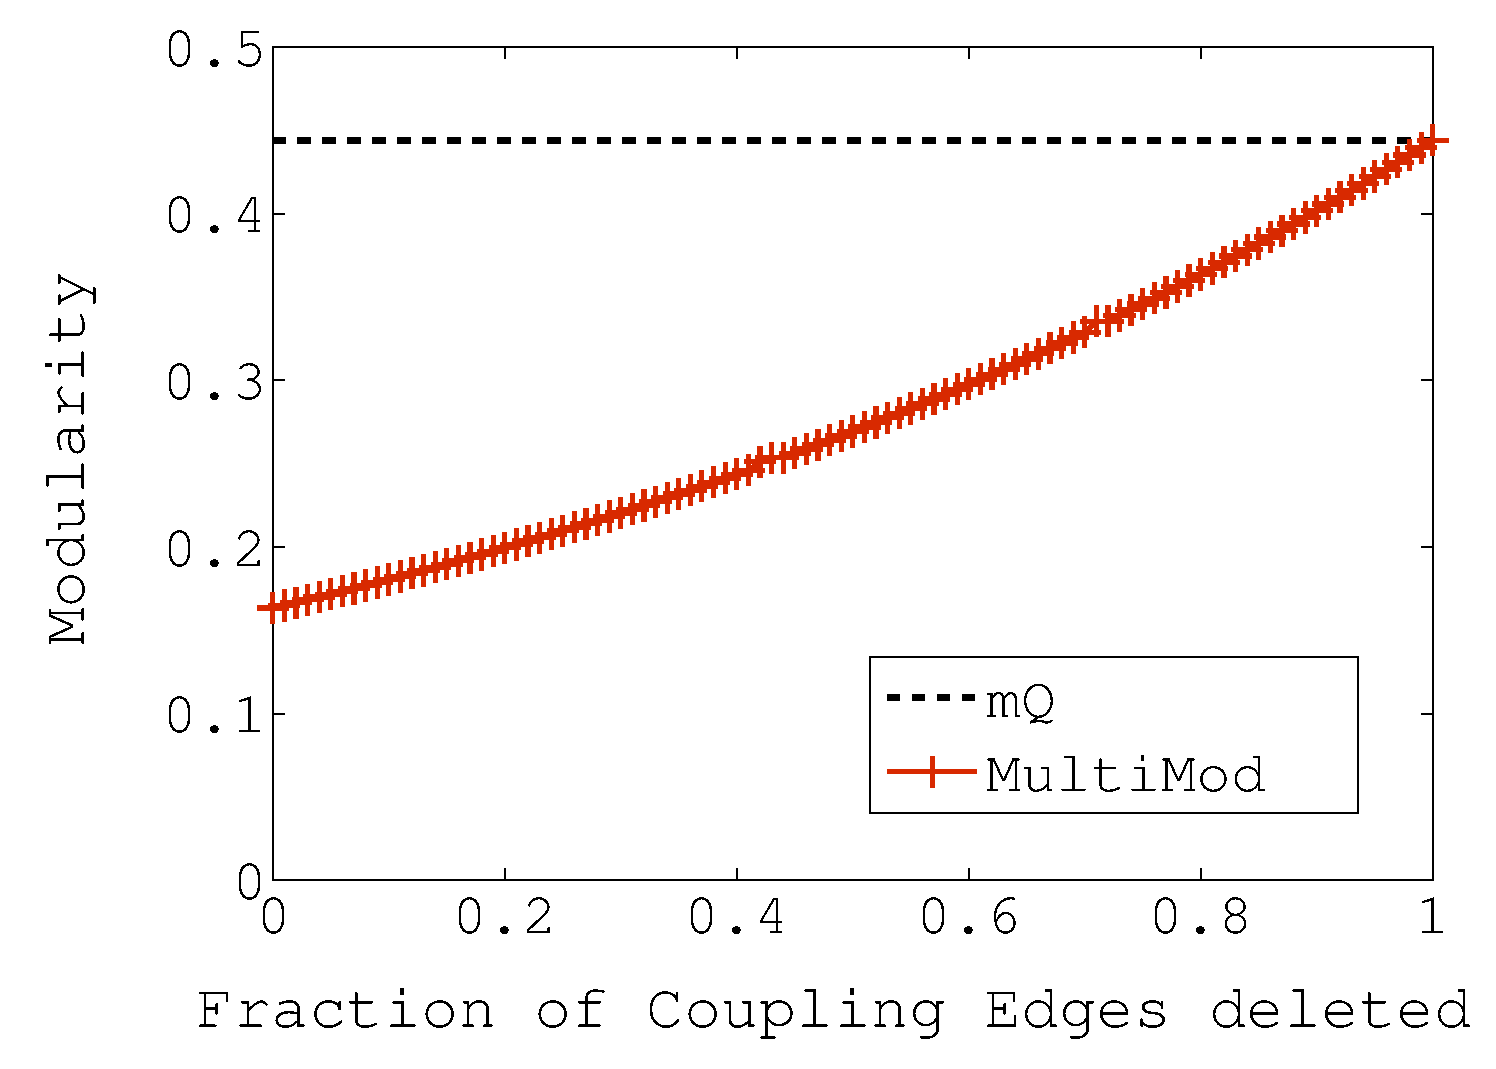
\includegraphics[angle=0,scale=.23]{./images/mQ_vs_single_config2_100_5_no_ext_random_removal.pdf}}
% % \subfigure[Config B
% % ]{\label{single0}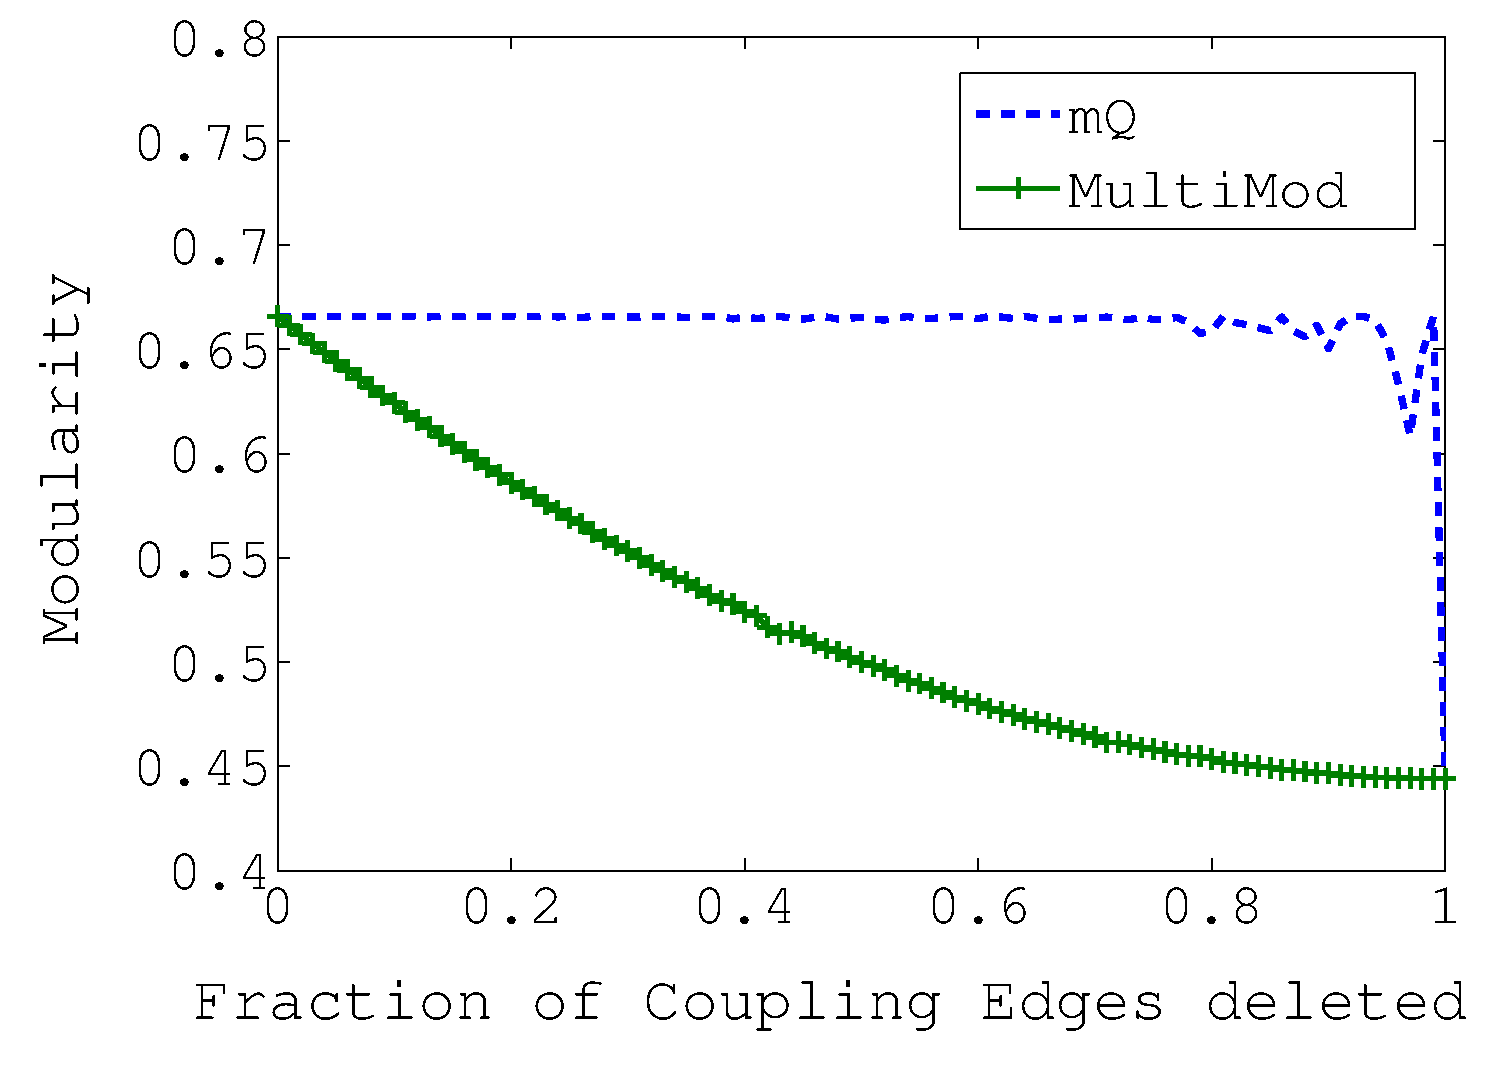
\includegraphics[angle=0,scale=.23]{./images/mQ_vs_single_config1_100_5_no_ext_random_removal.pdf}}
% % \end{center}
% % \vspace{-0.25in}
% % \caption{Change in mQ and MultiMod while deleting coupling edges for both Single layer (Config A) \& Multilayer (Config B) ground truth
% % communities in Fig.~\ref{N0}}
% % \vspace{-0.2in}
% % \label{single}
% % \end{figure*}
% %
% % where $F^C_1$  represents the fraction of $L^C_1$ nodes connected to at least one $L_2$ node from a different community;
% % $H^C_1$ represents the fraction of $L^C_1$ nodes connected to at least one node from $L^C_2$;
% % $F^C_2$ and $H^C_2$ are also defined in the same manner. We summarize the corrections next.
% %
% % (a) We introduce the factors $e^{-F^C_1}$ and $e^{-F^C_2}$, respectively with the corresponding single layer modularity terms.
% % Consider a community $L^C_1$ which is very cohesive in the $L_1$ layer itself, however a high fraction of
% % nodes in $L^C_1$ may also be connected with the nodes of some different community of layer $L_2$ through coupling
% % edges (high $F^C_1$); this should dilute the cohesiveness of community $L^C_1$ and penalize the overall modularity.
% % Hence, we introduce the factors $e^{-F^C_1}$ and $e^{-F^C_2}$ to penalize the single layer terms of modularity.
% % Fig.~\ref{single1} depicts that in Config A, modularity
% % $MultiMod$ gracefully improves as a result of removal of these type of coupling edges.
% %
% % (b) The factor $H^C_1\times H^C_2$, introduced with the coupling layer term of Eq.~\ref{eqn2}, measures how strongly the coupling
% % edges in community $C$ connect the group of nodes
% % $L^C_1$ and $L^C_2$ respectively. In Config B, even if the cross layer term results in high modularity, removal
% % of coupling edges results in low $H^C_1\times H^C_2$, which in turn reduces $MultiMod$. In Fig.~\ref{single0}, we can
% % observe that in Config B, $MultiMod$ gracefully degrades, following our intuition, with deletion
% % of coupling edges.
\subsection{Community detection algorithm}
We leverage on the single layer community detection algorithms Girvan-Newman~\cite{newman2004finding} \& Louvain~\cite{blondel2008fast}
which detect communities by maximizing Girvan-Newman modularity~\cite{newman2006modularity}.
%For example, in Girvan-Newman algorithm, we partition the network by removing edges in the descending order
%of their betweenness-centrality values and obtain the partition with highest modularity.
%Similar modularity maximization is adopted for Louvain too.

\vspace{-0.1in}
\begin{algorithm} \small

    \DontPrintSemicolon
    \SetKwInOut{Input}{Input}
    \SetKwInOut{Output}{Output}
    \SetKwProg{Fn}{Function}{:}{}
     \Input{A multilayer network $\mathcal{G}$ as defined in section~\ref{mult_mod} where $V= V_1 \cup V_2$.} 
%     is the set of all nodes in all the layers of $\mathcal{G}$.}
     \Output{Maximum $Q_M$ of $\mathcal{G}$ and detected communities.}

%      \ForEach{$node \in N_E \cup N_V$}{%
%       act[node]=0\;
%      }
% % \While{$\left \vert V \right \vert > 0$}{
% %      $oldQ$=-1\;
% %      $currQ$=0\;
% %      $Ite$=0\;
% %      $reassign$=0\;
% %      \While{$oldQ$ $\neq$ $currQ$ and $Ite < MaxIt$}{
% %       $oldQ$=$currQ$\;
% %       $currQ$=0\;
% %       $Ite=Ite+1$\;
% %       \ForEach{$v \in V$}{%
% % 	$currQ$ = current $Q_M$ of $G$\;
% % 	$Nei(v)$ = set of neighboring communities of $v$\;
% % 	
% % 	\ForEach{community $c \in Nei(v)$}{ %\textit{//Neighbours of $e_{max}$ in $X_E$}   \;
% % 	  Put $v$ into $c$\;
% % 	  $newQ$ = current $Q_M$ of $G$\;
% % 	  $gain_c$ = $newQ - currQ$
% % 	}
% % 	$c_{max}$ = Find $c \in Nei(v)$ with maximum $gain_c$\;
% % 	\uIf{$gain_{c_{max}} > 0$}{
% % 	    Assign $v$ to $c_{max}$\;
% % 	    $reassign=1$\;}
% % 	  \Else{
% % 	    Keep $v$ in its current community\;}
% % 	
% %  	
% %  	
% %        }
% %       $currQ$ = current $Q_M$ of $G$
% % }	
% % \If{$reassign==0$}
% %  	{break\;}
% %  $G$= Modify G by considering the detected communities as nodes and updating edges between them accordingly.	
% % }
% %      $currQ$ is the maximized $Q_M$\;

    \While{True}{
      Place each node of $\mathcal{G}$ into a single community\;
      Save $Q_M$ for this decomposition\;
      \While {there are moved nodes}{
	\ForEach{node $n \in V$}{
	    c = neighboring community of $n$ maximizing $Q_M$ increase\;
	    \If{c results in a strictly positive increase}{
	      move n from its community to c\;
	    }
	}
      }
      \uIf {$Q_M$ reached is higher than the initial $Q_M$}{
	Display the partition found\;
	Transform $\mathcal{G}$ into the network between communities\;
	}
      \Else{
	break\;
      }
    }
    \KwRet\;

\caption{Louvain-$Q_M$} %Algorithm to map Meetup venues with Yelp venues}
\label{algo2}
\end{algorithm}
\vspace{-0.1in}


We substitute the Girvan-Newman modularity by our proposed modularity index $Q_M$ and develop \textbf{GN-$Q_M$} (Algo.~\ref{algo3})
and \textbf{Louvain-$Q_M$} (Algo.~\ref{algo2}) algorithms respectively for multilayer networks.
Although vanilla algorithms are intrinsically incapable of distinguishing different types of edges and nodes in the multilayer 
network, however, due to
the adaptability of $Q_M$, \textbf{GN-$Q_M$} and \textbf{Louvain-$Q_M$} should be able to detect both cross layer
and single layer communities. Essentially $Q_M$ works as a patch on top of any single layer
community detection algorithm to detect multilayer communities.

% \begin{itemize}
%  \item \textbf{GN-$Q_M$}: In this algorithm (see Alg.~\ref{algo3}), at every step we remove an edge with the maximum
%  betweenness centrality until there are no edges left in the graph. During this process, we save the $Q_M$
%  value corresponding to each partition created after the edge removal and finally output the partition with the maximum $Q_M$ value.


% %  \item \textbf{Louvain-$Q_M$}: In this algorithm (see Algo.~\ref{algo2}), we begin with initializing
% % every node of the input network to a singleton community. A node is moved to a neighbouring community only if this movement results in a
% % strictly positive increase in $Q_M$ of the entire network. This process is repeated for each vertex and the iteration ends when no
% % other movement is possible. At the next pass, all the detected communities are considered as nodes (edges updated accordingly) and the
% % same process continues. The algorithm stops if there is no increase in $Q_M$ value in a particular pass and thereby, the most recent
% % partition is obtained as the output of the algorithm.
% % \end{itemize}

%
% Our algorithm is a heuristic, that strives to obtain a high value of $Q_M$. In this algorithm, we begin with initializing
% every vertex to a singleton community. A vertex is moved to a community only if this movement results in a
% net increase in $Q_M$ of the entire network.
% This process is repeated for each vertex and the iteration ends when no other movement is possible.
% At the next step all the detected communities are considered as vertices (edges updated accordingly) and the
% same process continues.
% This process is repeated for each vertex and the entire relocation of
% all vertices is repeated over several iterations until the $Q_M$ value converges.
% However, convergence is not theoretically guaranteed, but we empirically observe that the algorithm
% converges with high probability.

\subsection{Convergence \& Complexity}
Finally we show that algorithms \textbf{GN-$Q_M$} and \textbf{Louvain-$Q_M$}
converge and they are tractable in terms of time complexity.

\subsubsection{\textbf{GN-$Q_M$}} At every step we remove one edge from the network and hence, the algorithm certainly stops
after the removal of all the $\left \vert E_1 \right \vert + \left \vert E_{12} \right \vert+ \left \vert E_2 \right \vert$ edges.
Clearly, the theoretical worst case complexity of the algorithm is
$O((\left \vert V_1 \right \vert + \left \vert V_2 \right \vert)\times(\left \vert E_1 \right \vert +
\left \vert E_{12} \right \vert+ \left \vert E_2 \right \vert)^2)$ as finding betweenness centrality in unweighted graphs
costs $O((\left \vert V_1 \right \vert + \left \vert V_2 \right \vert)\times(\left \vert E_1 \right \vert +
\left \vert E_{12} \right \vert+ \left \vert E_2 \right \vert))$ operations~\cite{PhysRevE.64.016132}.
%\textcolor{red}{[SP:Please check. Ref needed?, JLG: Ok, ref is Newman M E J(2001) Phys Rev E 64:016131]}



\subsubsection{\textbf{Louvain-$Q_M$}} At each iteration of every pass, each node is placed
into one of its neighbouring community only if the movement leads to a
strictly positive gain in modularity $Q_M$. Computing this gain both proves
that the algorithms converges and gives an upper bound on its complexity.

Suppose, at any particular iteration the node $x$ is to be moved from its own
community $C_1$ to another community $C_2$. Without loss of generality, let us
assume that $x \in V_1$ and $x$ is connected with $h_x$ nodes in $V_1$ \& $c_x$
nodes in $V_2$. For simplicity, we perform this movement in two steps: first, we
remove $x$ from $C_1$ and keep it as an isolated community; second,
we insert $x$ into $C_2$. $C_1$ and $C_2$ can be either cross layer or
single layer communities, independently. Below we derive the gain assuming
$C_1$ is cross layer and $C_2$ is single layer. The other three cases can be
derived in a similar manner. Note that since the
modularity is an independent sum over all communities, the contribution of other communities
than $C_1$ and $C_2$ is not affected by the movement of $x$. Therefore we will only compute
the change of modularity of $C_1$ and $C_2$.

%This makes our approach heavily generic and flexible.
%In the next section, we compare the performance of our algorithm with different types of existing baseline algorithms.


%Similar to Eq.~\ref{final1},
The modularity $Q_M^{C_1,C_2}$, restricted to $C_1$ and $C_2$, before any movement can be simply expressed as,
$Q_M^{C_1,C_2} = Q_M^{C_1}+ Q_M^{C_2}$,
where $Q_M^{C_1}$ follows from Eq.~\ref{eq_multi} (as $C_1$ is cross layer) and $Q_M^{C_2}$ follows from Eq.~\ref{eq_single}
(as $C_2$ is single layer).
%\begin{dmath}\label{final2}
%Q_M= \frac{1}{3}\left[ {\forall i,j \in C_1}~\penalty0   \bigg \{
% \frac{1}{2\left \vert E_1 \right \vert }
% \sum_{i,j \in V_1}(A_{ij} - \penalty0 \frac{ (h_i * h_j)}
% {2\left \vert E_1 \right \vert})  \\
% +
% \frac{1}{2\left \vert E_1 \right \vert + 2\left \vert E_2 \right \vert + \left \vert E_{12} \right \vert} \penalty0
% \sum_{i \in V_1, j \in V_2}(A_{ij} - \frac{ ({c'}_i * {c'}_j)}
% {2\left \vert E_1 \right \vert + 2\left \vert E_2 \right \vert + \left \vert E_{12} \right \vert}) \\+
% \frac{1}{2\left \vert E_{2} \right \vert} \penalty0
% \sum_{i,j \in V_2}(A_{ij} -
% \frac{ (h_i * h_j)}{2\left \vert E_2 \right \vert })
%   \bigg \} \right] +
%\frac{1}{3}\left[ {\forall i,j \in C_2}~\penalty0   \bigg \{
% \frac{1}{2\left \vert E_1 \right \vert + \left \vert E_{12} \right \vert }
% \sum_{i,j \in V_1}(A_{ij} - \penalty0 \frac{ (h_i+c_i) * (h_j+c_j)}
% {2\left \vert E_1 \right \vert+ \left \vert E_{12} \right \vert})
%   \bigg \} \right] +   \frac{1}{3}\sum_{k=3}^{n_C} Q_M^{C_k}
%\end{dmath}

% % \begin{dmath}\label{final2}
% % %Q_M= \frac{1}{3}\left[ {\forall i,j \in C_1}~\penalty0   \bigg \{
% % % \frac{1}{2\left \vert E_1 \right \vert }
% % % \sum_{i,j \in V_1}(A_{ij} - \penalty0 \frac{ (h_i * h_j)}
% % % {2\left \vert E_1 \right \vert})  \\
% % % +
% % % \frac{1}{2\left \vert E_1 \right \vert + 2\left \vert E_2 \right \vert + \left \vert E_{12} \right \vert} \penalty0
% % % \sum_{i \in V_1, j \in V_2}(A_{ij} - \frac{ ({c'}_i * {c'}_j)}
% % % {2\left \vert E_1 \right \vert + 2\left \vert E_2 \right \vert + \left \vert E_{12} \right \vert}) \\+
% % % \frac{1}{2\left \vert E_{2} \right \vert} \penalty0
% % % \sum_{i,j \in V_2}(A_{ij} -
% % % \frac{ (h_i * h_j)}{2\left \vert E_2 \right \vert })
% % %   \bigg \} \right] +
% % %\frac{1}{3}\left[ {\forall i,j \in C_2}~\penalty0   \bigg \{
% % % \frac{1}{2\left \vert E_1 \right \vert + \left \vert E_{12} \right \vert }
% % % \sum_{i,j \in V_1}(A_{ij} - \penalty0 \frac{ (h_i+c_i) * (h_j+c_j)}
% % % {2\left \vert E_1 \right \vert+ \left \vert E_{12} \right \vert})
% % %   \bigg \} \right] +   \frac{1}{3}\sum_{k=3}^{n_C} Q_M^{C_k}
% % Q_M^{C_1,C_2}= \frac{1}{3}\left[
% %  \frac{1}{m_1} \sum_{i,j \in V_1,C_1} ( A_{ij} - \penalty0 \frac{h_i h_j}{m_1} ) +  \\
% %   \frac{1}{m} \penalty0
% %  \sum_{i \in V_1, j \in V_2, C_1}(A_{ij} - \frac{{c'}_i {c'}_j}{m}) +
% %  \frac{1}{m_2} \sum_{i,j \in V_2,C_1}(A_{ij} - \frac{h_i h_j}{m_2})
% %    \right] +\penalty0
% % \frac{1}{3}\left[
% %  \frac{1}{m_{12}} \sum_{i,j \in V_1,C_2}(A_{ij} - \frac{(h_i+c_i) (h_j+c_j)}{m_{12}})
% %   \right]
% % \end{dmath}

Once node $x$ is removed from $C_1$ and kept as an isolated community, the modularity sum of the $C_1$, $C_2$ and ${x}$ becomes,
%\textcolor{red}{[JL: Can you make the $+1/m$ from en of first line of the equation to go on the second line?]}
\vspace{-0.18in}
\begin{dmath*}\label{final3}
Q_M^{C_1,C_2,\{x\}}= \frac{1}{3}\left[
 \frac{1}{m_1} \sum_{i,j \in V_1 ,C_1 - \{x\}} \big(A_{ij} - \penalty0 \frac{h_i h_j}{m_1}\big) +\\
 {\frac{1}{m}  \sum_{i,j \in  C_1 - \{x\}, i \in V_1, j \in V_2} \big(A_{ij} - \frac{ {c'}_i {c'}_j}{m}\big) +
 \frac{1}{m_2}} \penalty0 \sum_{i,j \in V_2,C_1 - \{x\}} \big(A_{ij} - \frac{h_i h_j}{m_2}\big) \right] +  
 \frac{1}{3}\left[ \frac{1}{m_{21}} \penalty0 \big(A_{xx} - \frac{(h_x+c_x)^2}{m_{21}}\big)\right] + Q_M^{C_2}
 %\frac{1}{3}\left[ \frac{1}{m_{12}} \sum_{i,j \in V_1,C_2} (A_{ij} - \frac{(h_i+c_i)(h_j+c_j)}{m_{12}}) \right]
\end{dmath*}
\vspace{-0.05in}
where $m_1=2\left \vert E_1 \right \vert$, $m_2=2\left \vert E_2 \right \vert$,
$m_{12} = 2\left \vert E_1 \right \vert + \left \vert E_{12} \right \vert$, $m_{21} = 2\left \vert E_2 \right \vert + \left \vert E_{12} \right \vert$ and
$m=2\left \vert E_1 \right \vert + 2\left \vert E_2 \right \vert + \left \vert E_{12} \right \vert$.

Hence, the change in modularity $\Delta_r=Q_M^{C_1,C_2,\{x\}}-Q_M^{C_1,C_2}$ due to this removal (assuming $A_{xx} = 0$) is the following,
\vspace{-0.05in}
\begin{dmath*}\label{final4}
\Delta_r = \frac{h_x^2}{3{m_1}^2} -
  \frac{1}{3}\left[
    \frac{1}{m_1} \sum_{i \in V_1, C_1 - \{x\}} \big(A_{ix} - \frac{(h_i h_x)}{m_1}\big) +
    \frac{1}{m} \sum_{i \in V_2, C_1 - \{x\}} \big(A_{xi} - \frac{ {c'}_x  {c'}_i}{m}\big)
    \right] - \frac{ (h_x+c_x)^2}{3m_{21}^2}
% \Delta_{removal} = Q_M^{'}-Q_M = -
%\frac{1}{3}\left[ {\forall i \in C_1 - \{x\}}~\penalty0   \bigg \{
% \frac{1}{2\left \vert E_1 \right \vert }
% \sum_{i \in V_1}(A_{ix} - \penalty0 \frac{ (h_i * h_x)}
% {2\left \vert E_1 \right \vert})  \\
% +
% \frac{1}{2\left \vert E_1 \right \vert + 2\left \vert E_2 \right \vert + \left \vert E_{12} \right \vert} \penalty0
% \sum_{i \in V_2}(A_{xi} - \frac{ ({c'}_x * {c'}_i)}
% {2\left \vert E_1 \right \vert + 2\left \vert E_2 \right \vert + \left \vert E_{12} \right \vert})\bigg \} \right] -
%  \frac{1}{3}\left[
% \frac{ (h_x+c_x)^2}{(2\left \vert E_2 \right \vert + \left \vert E_{12} \right \vert)^2}\right]
% + \frac{h_x^2}{3.(2\left \vert E_1 \right \vert)^2}
\end{dmath*}
\vspace{-0.05in}

%After inserting $x$ into $C_2$, $Q_M$ can be expressed as,
%\begin{dmath}\label{final5}
%Q_M^{''}= \frac{1}{3}\left[ {\forall i,j \in C_1 - \{x\}}~\penalty0   \bigg \{
% \frac{1}{2\left \vert E_1 \right \vert }
% \sum_{i,j \in V_1}(A_{ij} - \penalty0 \frac{ (h_i * h_j)}
% {2\left \vert E_1 \right \vert})  \\
% +
% \frac{1}{2\left \vert E_1 \right \vert + 2\left \vert E_2 \right \vert + \left \vert E_{12} \right \vert} \penalty0
% \sum_{i \in V_1, j \in V_2}(A_{ij} - \frac{ ({c'}_i * {c'}_j)}
% {2\left \vert E_1 \right \vert + 2\left \vert E_2 \right \vert + \left \vert E_{12} \right \vert}) +
% \frac{1}{2\left \vert E_{2} \right \vert} \penalty0
% \sum_{i,j \in V_2}(A_{ij} -
% \frac{ (h_i * h_j)}{2\left \vert E_2 \right \vert })
%   \bigg \} \right] +
%\frac{1}{3}\left[ {\forall i,j \in C_2+\{x\}}~\penalty0   \bigg \{
% \frac{1}{2\left \vert E_1 \right \vert + \left \vert E_{12} \right \vert }
% \sum_{i,j \in V_1}(A_{ij} - \penalty0 \frac{ (h_i+c_i) * (h_j+c_j)}
% {2\left \vert E_1 \right \vert+ \left \vert E_{12} \right \vert})
%   \bigg \} \right]
% +  \frac{1}{3}\sum_{k=3}^{n_C} Q_M^{C_k}
%\end{dmath}

Similarly, the change in modularity $\Delta_i$ due to the insertion of $x$ in
$C_2$ can be computed as,
\vspace{-0.05in}
\begin{dmath*}\label{final6}
\Delta_{i} =
 \frac{1}{3m_{12}}
 \sum_{i \in V_1, C_2}\big(A_{ix} - \frac{ (h_i+c_i)(h_x+c_x)}{m_{12}}\big)+\frac{ (h_x+c_x)^2}{3m_{21}^2}
\end{dmath*}
\vspace{-0.05in}
Finally, the overall improvement due to this movement of node $x$ from
community $C_1$ to community $C_2$ is\footnote{Same order of magnitude can
be derived for other types of $C_1$ and $C_2$.},
\vspace{-0.05in}
\begin{dmath*}\label{final7}
\Delta_{r}+\Delta_{i} = \Theta(\frac{1}{m^2})
% Q_M^{''}-Q_M =
%\Delta_{removal}+\Delta_{insertion} = -
%\frac{1}{3}\left[ {\forall i \in C_1 - \{x\}}~\penalty0   \bigg \{
% \frac{1}{2\left \vert E_1 \right \vert }
% \sum_{i \in V_1}(A_{ix} - \penalty0 \frac{ (h_i * h_x)}
% {2\left \vert E_1 \right \vert})  \\
% +
% \frac{1}{2\left \vert E_1 \right \vert + 2\left \vert E_2 \right \vert + \left \vert E_{12} \right \vert} \penalty0
% \sum_{i \in V_2}(A_{xi} - \frac{ ({c'}_x * {c'}_i)}
% {2\left \vert E_1 \right \vert + 2\left \vert E_2 \right \vert + \left \vert E_{12} \right \vert})\bigg \} \right]
% + \frac{h_x^2}{3.(2\left \vert E_1 \right \vert)^2} +\frac{1}{3}\left[ {\forall i \in C_2}~\penalty0   \bigg \{
% \frac{1}{2\left \vert E_1 \right \vert + \left \vert E_{12} \right \vert }
% \sum_{i \in V_1}(A_{ix} - \penalty0 \frac{ (h_i+c_i) * (h_x+c_x)}
% {2\left \vert E_1 \right \vert+ \left \vert E_{12} \right \vert})
%   \bigg \} \right]
%   \geq \frac{1}{({2\left \vert E_1 \right \vert + 2\left \vert E_2 \right \vert +
%\left \vert E_{12} \right \vert})^2}
\end{dmath*}
\vspace{-0.05in}

Since the minimum gain for every move is of the order of $1/m^2$, in the worst
case we need $O(m^2)$ iterations to maximize $Q_M$ (as it is comprised between -1 and 1).
%As each iteration considers every vertex once, it leads to
%$O({\left \vert V_1 \right \vert + \left \vert V_2 \right \vert})$ operations
%per iteration. The theoretical worst case complexity of \textbf{Louvain-$Q_M$}  is therefore
%$O(({\left \vert V_1 \right \vert + \left \vert V_2 \right \vert})m^2)$.
%\textcolor{red}{[JL: we forgot the cost for computing the best neighboring community, we can cite Louvain directly or the below paper]}
We apply the same technique as in~\cite{blondel2008fast} to find the best neighboring community, so the cost for one vertex
is proportional to its degree. As each iteration considers every vertex once, it leads to $O(m)$ operations per iteration. The
theoretical worst case complexity of \textbf{Louvain-$Q_M$} is therefore $O(m^3)$.
In practice, this worst case complexity bound is quite loose. For instance, in
Fig.~\ref{gain}, we show the fraction of nodes moved along with the gain in
modularity in each iteration of the first pass of the \textbf{Louvain-$Q_M$} algorithm
while running it on a synthetic two layer network (generated following section~\ref{syn_gen}). The network has $600$ nodes ($300$ in
each layer) with $29,738$ edges ($m^2 = 1,104,232,900$) and the theoretical number of iterations could be of the
order 1 billion but it takes just $5$ iterations to end the first pass.

% \begin{figure}
% \centering
% 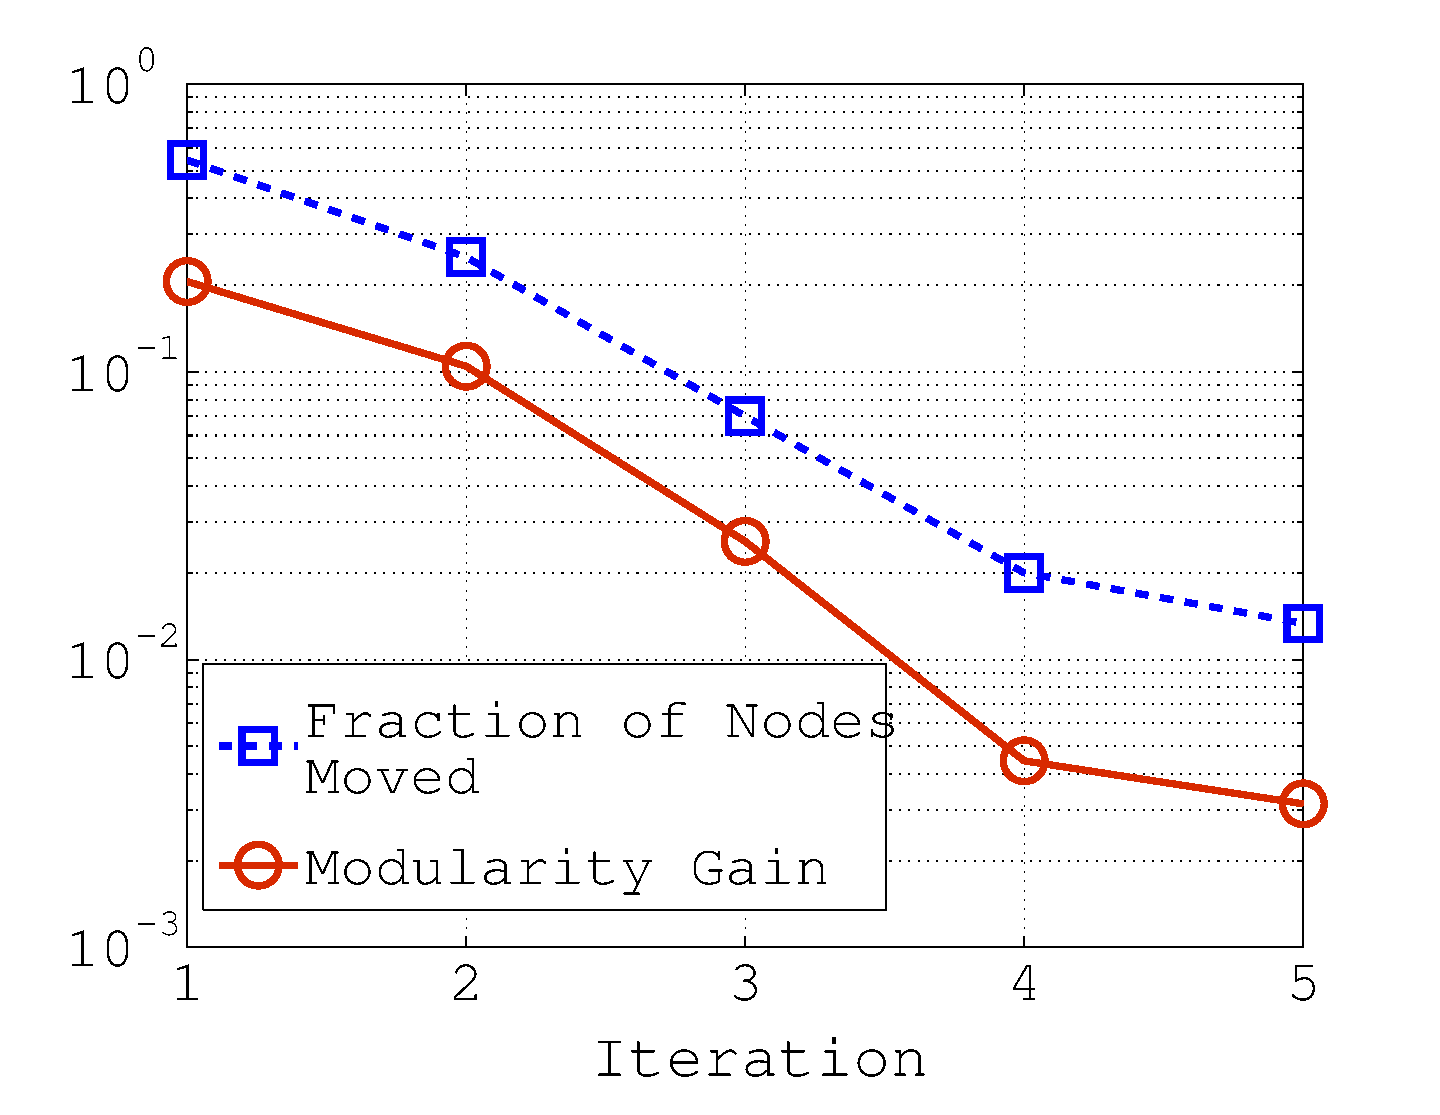
\includegraphics[width=2in]{./images/gain_drop.pdf}
% \vspace{-0.12in}
% \caption{Drop in modularity gain along with fraction of modes moved in the first pass of \textbf{Louvain-$Q_M$} for a $300\times300$
% synthetic multilayer network.}
% \vspace{-0.15in}
% \label{gain}
% \end{figure}


\begin{figure*}
\begin{center}
\subfigure[Drop in modularity gain with number of iterations.
]{\label{gain}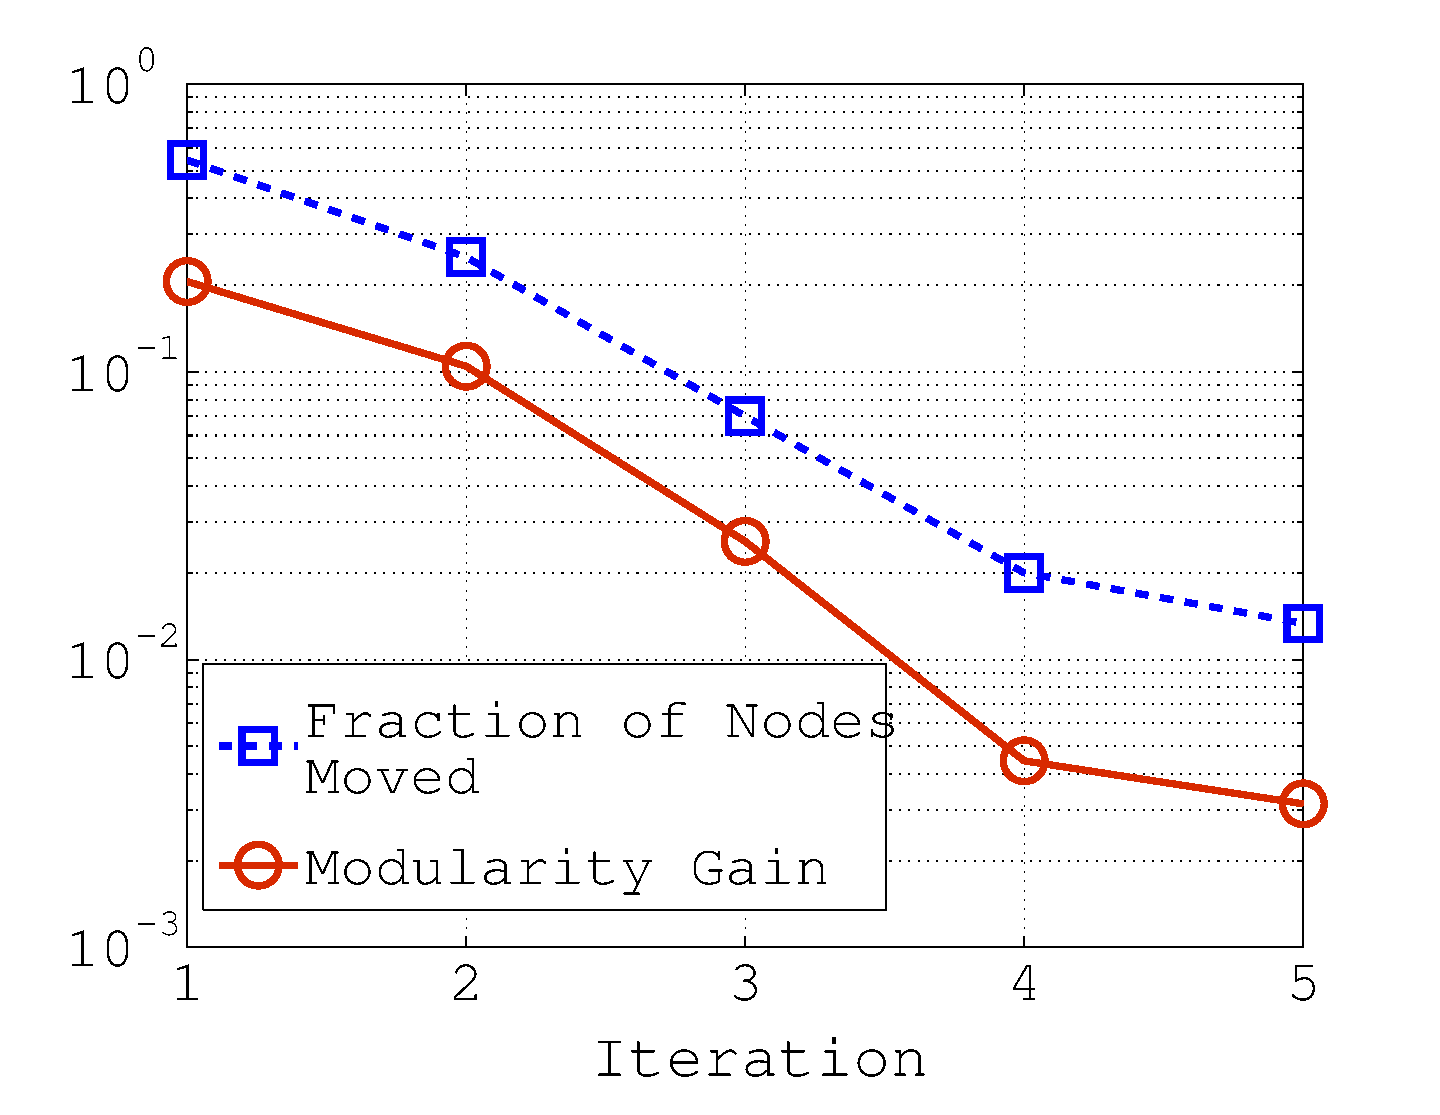
\includegraphics[angle=0,scale=.18]{./images/gain_drop.pdf}}
\subfigure[$mQ$ vs. $Q_M$ for Config A while adding coupling links.
]{\label{cross_single}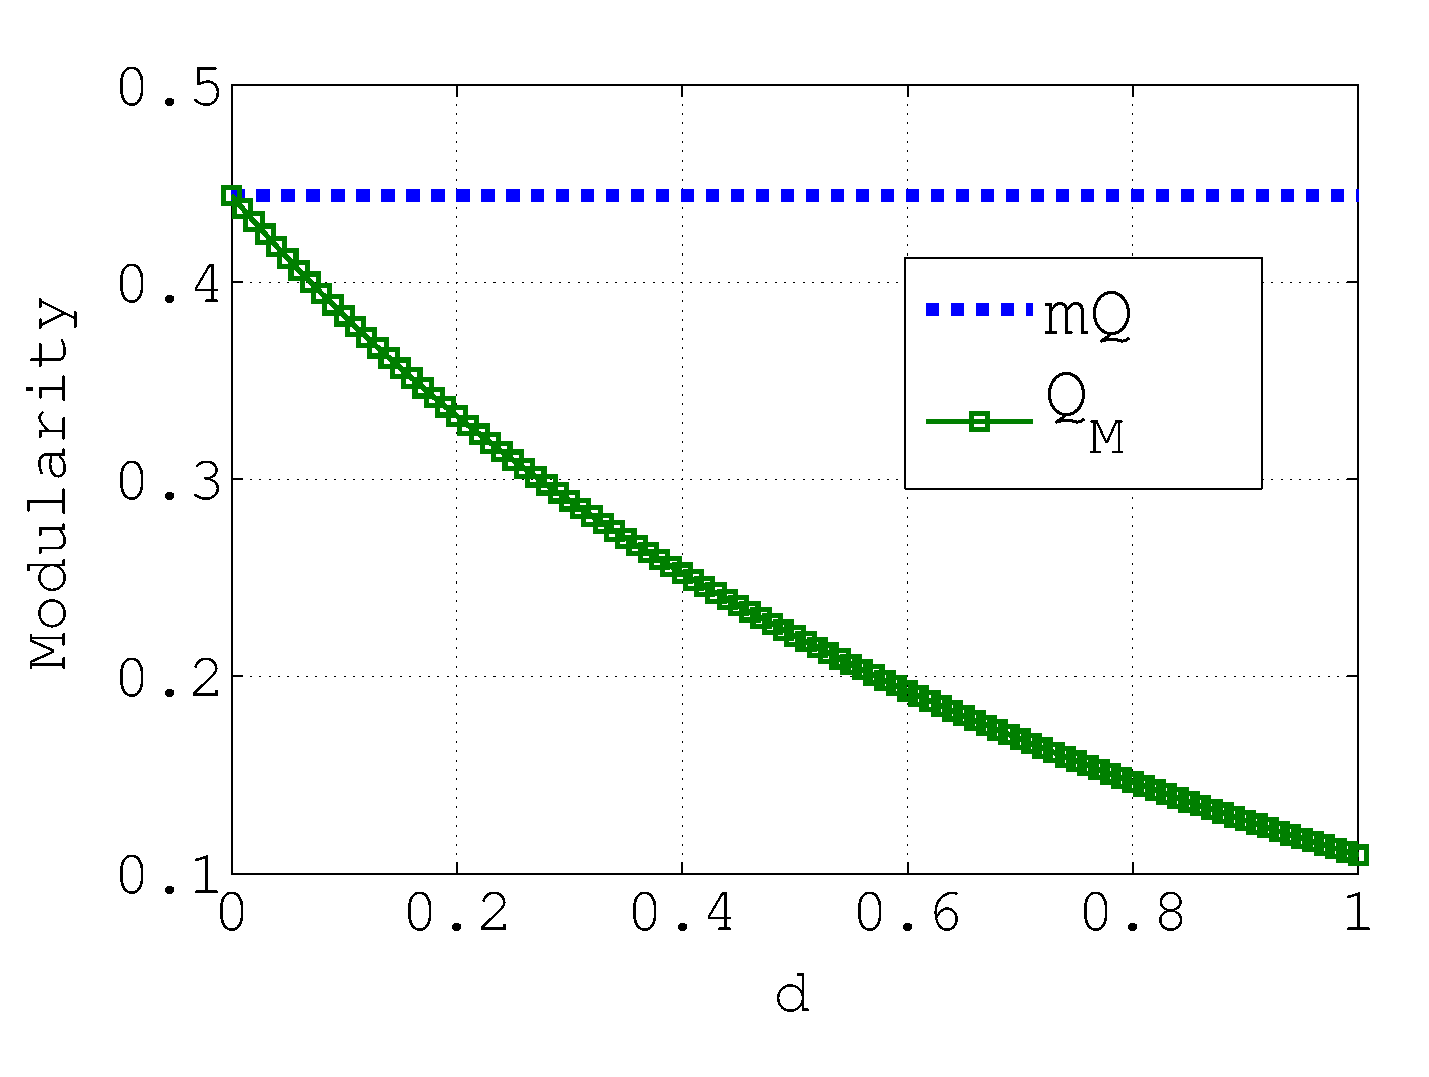
\includegraphics[angle=0,scale=.18]{./images/mQ_vs_march21_cross_single_square.pdf}}
\subfigure[$mQ$ vs. $Q_M$ for Config B while adding coupling links with varying $p$.
]{\label{cross_multi}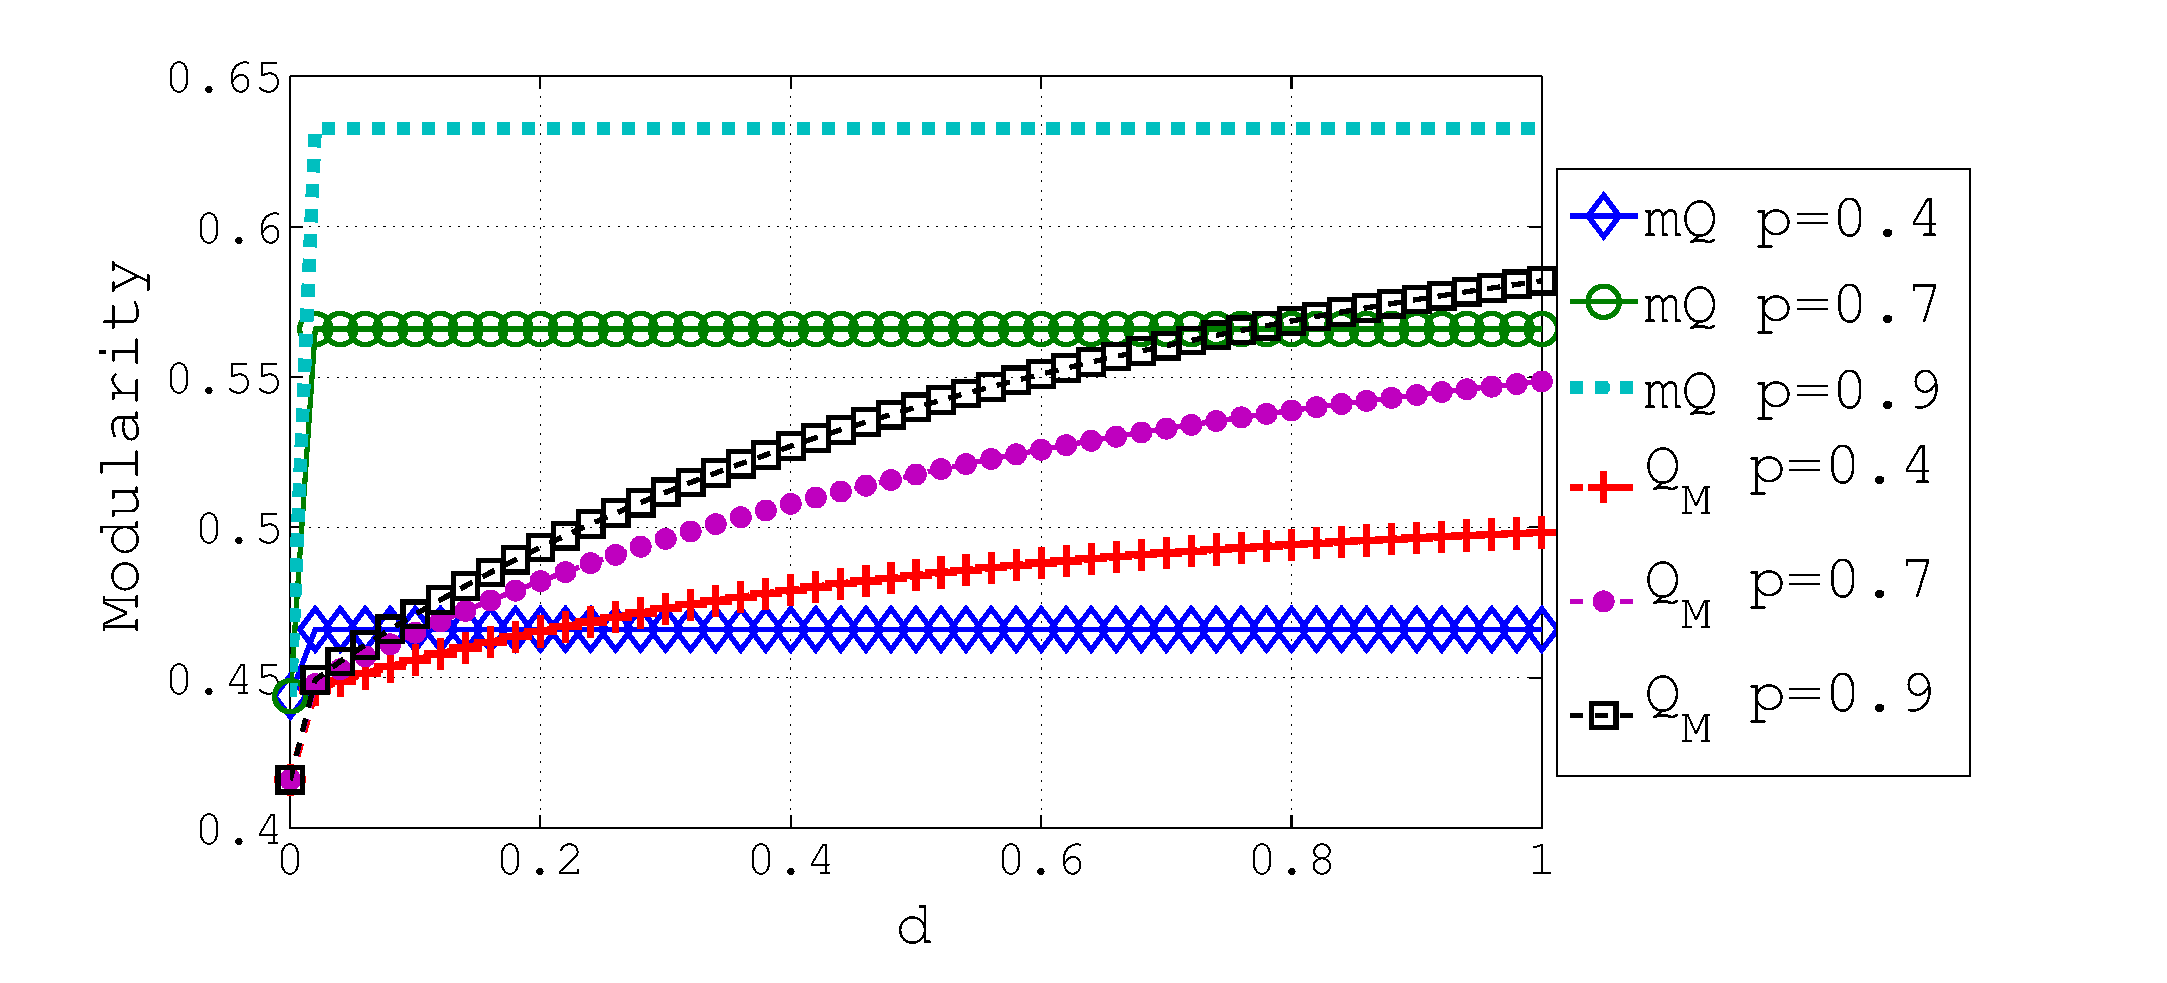
\includegraphics[angle=0,scale=.18]{./images/mQ_vs_march21_cross_multi.pdf}}
\end{center}
\vspace{-0.24in}
\caption{(a) Drop in modularity gain along with fraction of modes moved in the first pass of \textbf{Louvain-$Q_M$} for a $300\times300$
synthetic multilayer network; (b) \& (c) Comparative results
of $Q_M$ \& $mQ$ on the configurations in Fig.~\ref{N0}.}
\vspace{-0.22in}
\label{cross_multi_single}
\end{figure*}

